\documentclass[../main.tex]{subfiles}
\begin{document}
\begin{warningbox}
Rechte werden unterschieden in juridische (deontisch, dynamisch, vor dem Staat) und moralischen (\textit{sind} da), die uns unter Pflichten und Rechte stellen, die wir gemäss der Willenstheorie immer (wenn mündig) beherrschen können und gemäss der Interessenstheorie nur dann, wenn sie den Interessen dienen. 
\end{warningbox}

 
Rechte werden unterschieden in zwei Kategorien: juridische und moralische Rechte.
 
\paragraph{Juridische Rechte} werden durch das Gesetz festgelegt und den Staat garantiert. Wir sind rechtlich geboten, sie zu respektieren. 
 
Sie bilden ein System von Normen, das heisst sie gebieten, verbieten und erlauben bestimmte Dinge. Der Konflikt dieser Normen kann dabei nicht ausgeschlossen werden. Zusätzlich müssen diese Normen sozial wirksam (angewendet) sein, ansonsten ist sie ungültig. Eine Norm ist also sozial wirksam, wenn ihr zugestimmt, sie befolgt und schlussendlich durchgesetzt wird.
 
Erzeugt werden juridische Normen in einer bestimmten Weise durch ein befugtes Organ. Sie können dynamisch weiterentwickelt werden. 
 
\paragraph{Moralische Rechte} sind durch die Moral gegeben. Auch sie bilden ein System von Rechten. Entgegen den juridischen Rechten gelten sie aber unabhängig von ihrer sozialen Wirksamkeit. D.h. sie bestehen auch, wenn alle sie ignorieren. Ebenfalls unterschiedlich ist ihre Erzeugung; Sie werden nicht erzeugt, sondern bestehen. Sie können also auch nicht dynamisch angepasst werden. 
 
\subsection{Moralische vs juridische Rechte}
 Moralische Rechte und juridische können, müssen sich jedoch nicht überschneiden. 
 
\subsection{Hohfeld's Arten von Rechten}
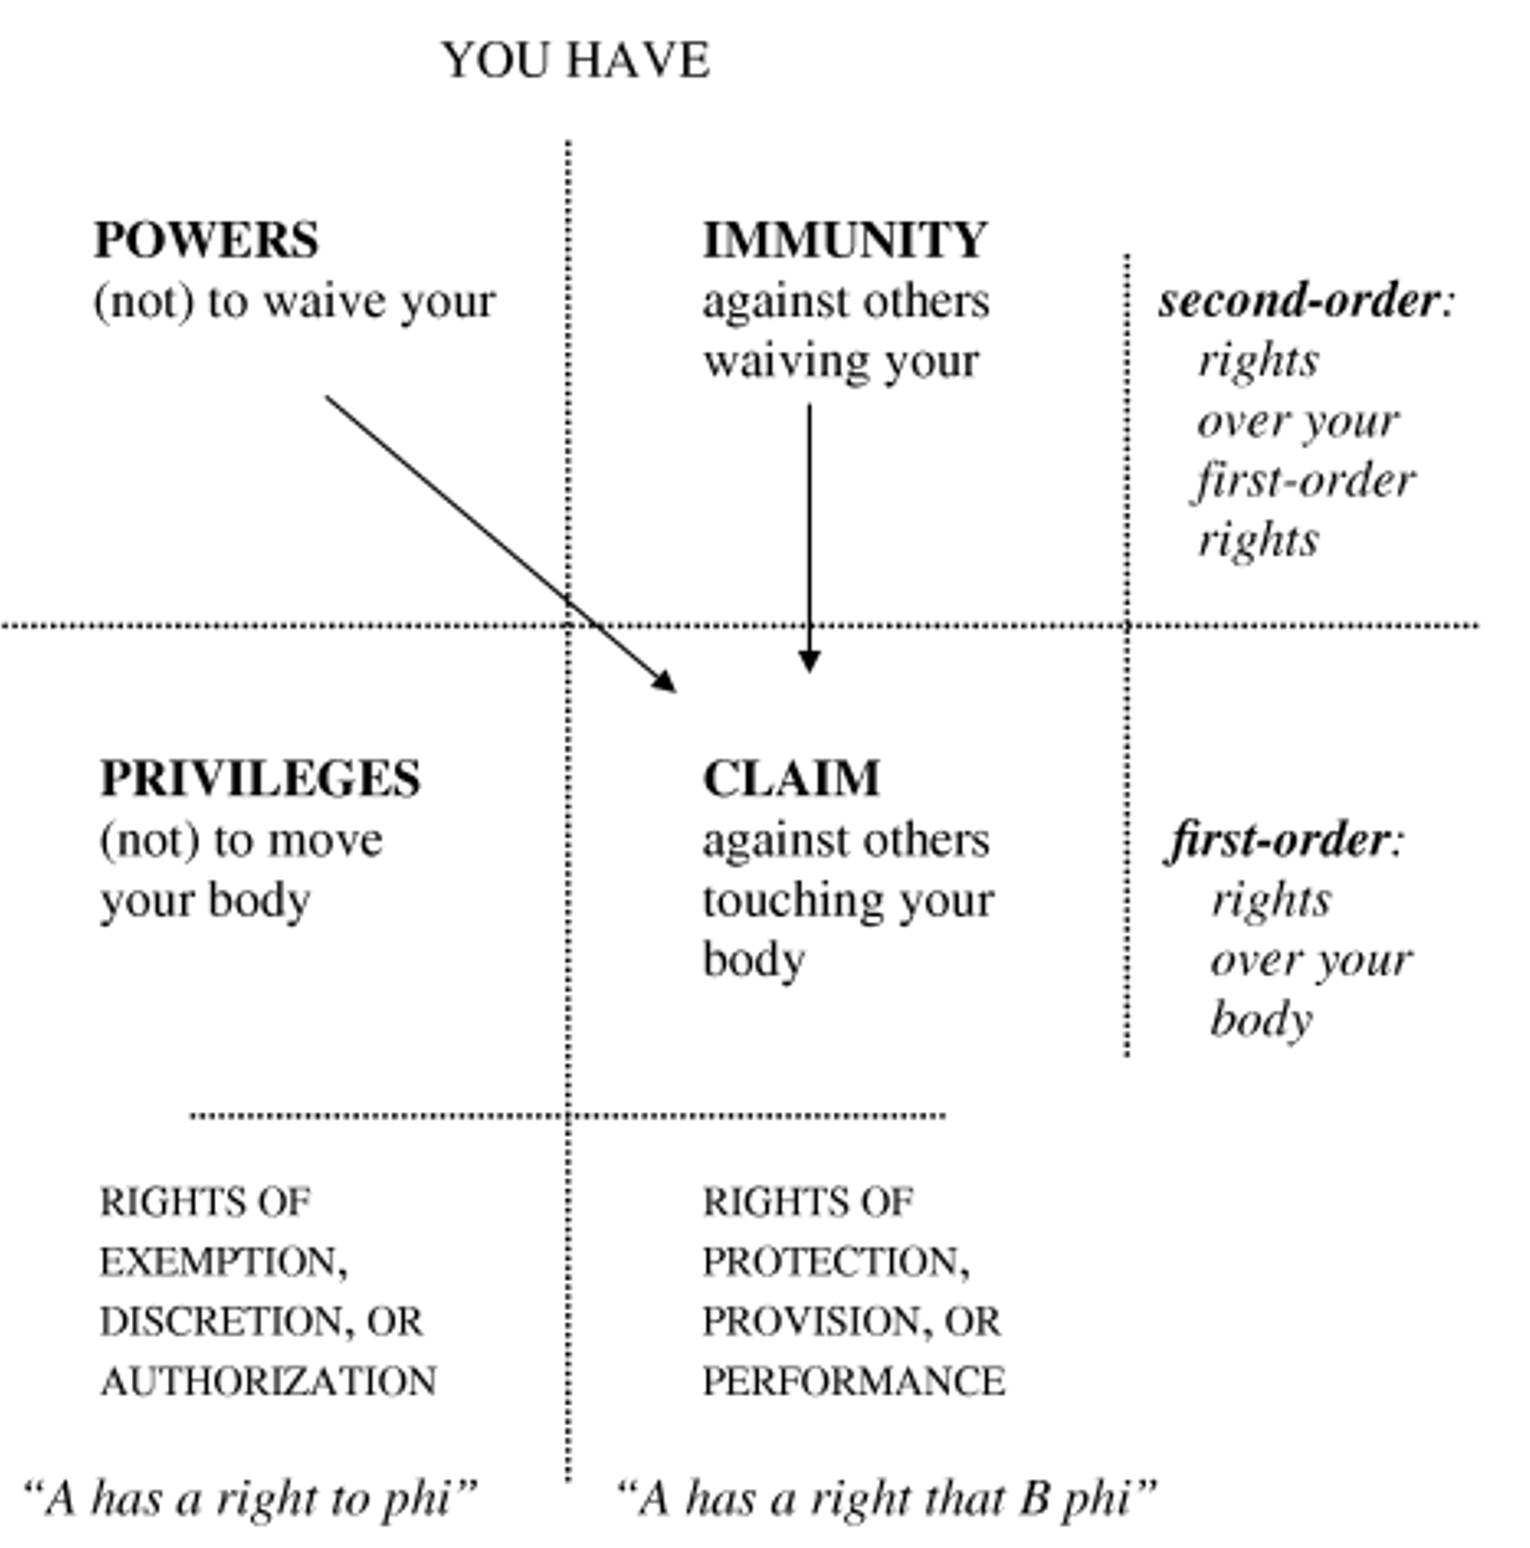
\includegraphics[width=\textwidth]{images/hohfelds_rights.png}

\paragraph{Privilegien} zu haben bedeutet, dass man nicht verpflichtet ist, etwas zu tun. Man ist frei, etwas zu tun, ohne bei Unterlass verurteilt werden zu können. 
\paragraph{Immunität} zu haben bedeutet, dass andere nicht in der Lage sind, die normative Situation von einem zu verändern. 
\paragraph{Power} zu besitzen bedeute, dass man in der Lage ist, die eigene normative Situation zu verändern.
\paragraph{Anspruchsrechte} zu besitzen bedeutet, dass man gegenüber einer anderen Person ein Recht hat, dass diese etwas unterlässt. Man hat also ein Recht darauf, dass jemand etwas nicht tut, resp. jemand hat die Pflicht, etwas nicht zu tun. Man könnte also sagen, dass Anspruchsrechten Pflichten (Handlungs- wie auch Unterlassungspflichten) korrespondieren. 

\subsection{Hart's Willenstheorie der Rechte}
\begin{warningbox}
Ein Recht zu haben heisst nach der Willenstheorie, dass andere eine
Pflicht haben, die von der Rechtsträgerin kontrolliert werden kann.	
\end{warningbox}

Gemäss H.L.A.Hart (1907-1992) bedeutet ein Recht zu haben, die Pflicht anderer kontrollieren zu können. So kann man, wenn man sagt, dass jemand das eigene Grundstück nicht betreten darf, dessen Pflicht, dieses nicht zu betreten, entweder so belassen oder ihn aus dieser entlassen. Dies nennt man \textit{legal powers}. Sie ermöglichen dem Träger des Rechts die Pflichten anderer ausser Kraft zu setzten oder das Recht zu transferieren. Im Falle von juridischen Rechten entsteht bei Rechtsverstoss die Möglichkeit zu klagen. 

Die Willenstheorie funktioniert nur mit Menschen, die ihr Recht beherrschen können. Dadurch entstehen jedoch Schwierigkeiten, da Trägerinnen von Rechten nur Menschen sein können, die diese Formen der Pflichtkontrolle ausüben können. Andere Wesen sind ausgeschlossen. Zusätzlich sollte gemäss der Willenstheorie jedes Recht ausser Kraft setzbar oder transferierbar sein (z.B. Folter). Dies schneidet sich mit der Idee von \textit{unveräusserlichen Rechten}.

\subsection{Die Interessenstheorie der Rechte}
\begin{warningbox}
Ein Recht zu haben heisst nach der Interessentheorie, dass andere unter einer dem Recht korrespondierenden Pflicht stehen.	
\end{warningbox}

Gemäss der Interessenstheorie schützen Rechte lediglich die Interessen der sie tragenden Wesen, die gewichtig genug sind, andere unter eine Pflicht zu stellen. Dabei sind Interessen definiert als etwas, das \textit{gut} für das Wesen ist und Personen üblicherweise haben. 

Somit schützt die Interessentheorie auch die Rechte von Tieren, Kleinkindern und geistig Beeinträchtigten. Zusätzlich erlaubt diese Theorie die Unveräusserlichbarkeit von Rechten. Es stellt sich jedoch die Frage, wie sie mit den Interessen Dritter umgeht; Hat Person A, die auf Bitte von Person B auf Person C aufpasst, nur eine Verpflichtung gegenüber B oder auch gegenüber C?

% TODO Verpflichtung gegenüber Drittpersonen nicht ganz verstanden...


\end{document}